% Préambule commun des schémas TikZ (compilés séparément par construire_figures.py)
\documentclass[tikz,border=3pt]{standalone}
\usepackage[T1]{fontenc}
\usepackage[utf8]{inputenc}
\usepackage{lmodern}
\usepackage{amsmath,amssymb}
\usepackage{bm}
\usepackage[american,siunitx,straightvoltages]{circuitikz}
\usetikzlibrary{arrows.meta,positioning,calc,decorations.pathmorphing,
  decorations.markings,decorations.pathreplacing,patterns,shapes.geometric,
  shapes.misc,shapes.multipart,fit,backgrounds,3d,intersections,matrix}

\ctikzset{bipoles/length=1.1cm, amplifiers/scale=0.85, tripoles/op amp/width=1.4}

\tikzset{
  >={Latex[length=2mm,width=1.4mm]},
  every picture/.style={line width=0.6pt, font=\small},
  % schémas-blocs
  bloc/.style={draw, minimum width=1.5cm, minimum height=0.9cm, align=center,
               inner sep=3pt, fill=white},
  somme/.style={draw, circle, minimum size=4.5mm, inner sep=0pt, fill=white,
                path picture={\draw (path picture bounding box.north west)
                  -- (path picture bounding box.south east)
                  (path picture bounding box.north east)
                  -- (path picture bounding box.south west);}},
  gain/.style={draw, isosceles triangle, isosceles triangle apex angle=60,
               minimum size=8mm, inner sep=1pt, fill=white},
  bruit/.style={draw, circle, minimum size=4.5mm, inner sep=0pt, fill=white,
                path picture={\node at (path picture bounding box.center)
                  {\scriptsize$\ast$};}},
  cadre/.style={draw, dashed, rounded corners=1pt},
  cadrept/.style={draw, dash dot, rounded corners=1pt},
  fleche/.style={->},
  % mécanique
  bati/.style={pattern=north east lines, draw=none},
  ressort/.style={decorate, decoration={coil, aspect=0.4, segment length=2.2mm,
                  amplitude=2mm, pre length=2mm, post length=2mm}},
  zigzag/.style={decorate, decoration={zigzag, segment length=2mm,
                  amplitude=1.6mm, pre length=2mm, post length=2mm}},
  pivot/.style={draw, circle, fill=white, minimum size=2.2mm, inner sep=0pt},
  masse/.style={draw, fill=gray!25, minimum width=1.4cm, minimum height=0.8cm},
  cote/.style={<->, line width=0.4pt},
  axe/.style={->, line width=0.6pt},
  trait mixte/.style={dash dot, line width=0.4pt},
}

% Encastrement / bâti hachuré : \bati{(x1,y1)}{(x2,y2)} trace une ligne et ses hachures dessous
\newcommand{\bati}[3][0.18]{%
  \fill[pattern=north east lines] #2 rectangle ($#3+(0,-#1)$);
  \draw[line width=0.8pt] #2 -- #3;}

% Transducteur (deux cercles entrelacés) : \pic (t) at (x,y) {transducteur};  -> (t-o) entrée, (t-e) sortie
\tikzset{
  transducteur/.pic={\draw (-0.13,0) circle (0.24); \draw (0.13,0) circle (0.24);
    \coordinate (-o) at (-0.37,0); \coordinate (-e) at (0.37,0);
    \coordinate (-n) at (0,0.24); \coordinate (-s) at (0,-0.24);},
  bobine/.style={decorate, decoration={coil, aspect=0.7, segment length=1.4mm,
                 amplitude=1.6mm, pre length=1mm, post length=1mm}},
  sourcebruit/.style={draw, circle, minimum size=5mm, inner sep=0pt, fill=white,
                 label={[inner sep=0pt]center:$\ast$}},
  sourcecourant/.style={draw, circle, minimum size=5mm, inner sep=0pt, fill=white,
                 label={[inner sep=0pt]center:$\circledast$}},
}

% Composants compacts (pour les petits boîtiers des schémas-blocs)
\newcommand{\resistance}[2]{% de #1 à #2 (quelconque)
  \draw #1 -- ($#1!0.22!#2$) ($#1!0.78!#2$) -- #2;
  \draw[decorate, decoration={zigzag, segment length=1.5mm, amplitude=1.1mm}]
    ($#1!0.22!#2$) -- ($#1!0.78!#2$);}
\newcommand{\condensateur}[2]{% horizontal de #1 à #2
  \draw #1 -- ($($#1!0.5!#2$)+(-0.05,0)$) ($($#1!0.5!#2$)+(0.05,0)$) -- #2;
  \draw[line width=1pt] ($($#1!0.5!#2$)+(-0.05,0.14)$) -- ($($#1!0.5!#2$)+(-0.05,-0.14)$)
                        ($($#1!0.5!#2$)+(0.05,0.14)$) -- ($($#1!0.5!#2$)+(0.05,-0.14)$);}
% R // C horizontal : \RparC{(x,y)}{longueur}{écart}  (centre, longueur totale, écart vertical)
\newcommand{\RparC}[3]{%
  \coordinate (rcA) at ($#1+(-#2/2,0)$); \coordinate (rcB) at ($#1+(#2/2,0)$);
  \draw (rcA) -- ++(0.15,0) coordinate (rcA1) (rcB) -- ++(-0.15,0) coordinate (rcB1);
  \draw (rcA1) -- ++(0,#3/2) (rcA1) -- ++(0,-#3/2) (rcB1) -- ++(0,#3/2) (rcB1) -- ++(0,-#3/2);
  \resistance{($(rcA1)+(0,#3/2)$)}{($(rcB1)+(0,#3/2)$)}
  \condensateur{($(rcA1)+(0,-#3/2)$)}{($(rcB1)+(0,-#3/2)$)}}

\begin{document}
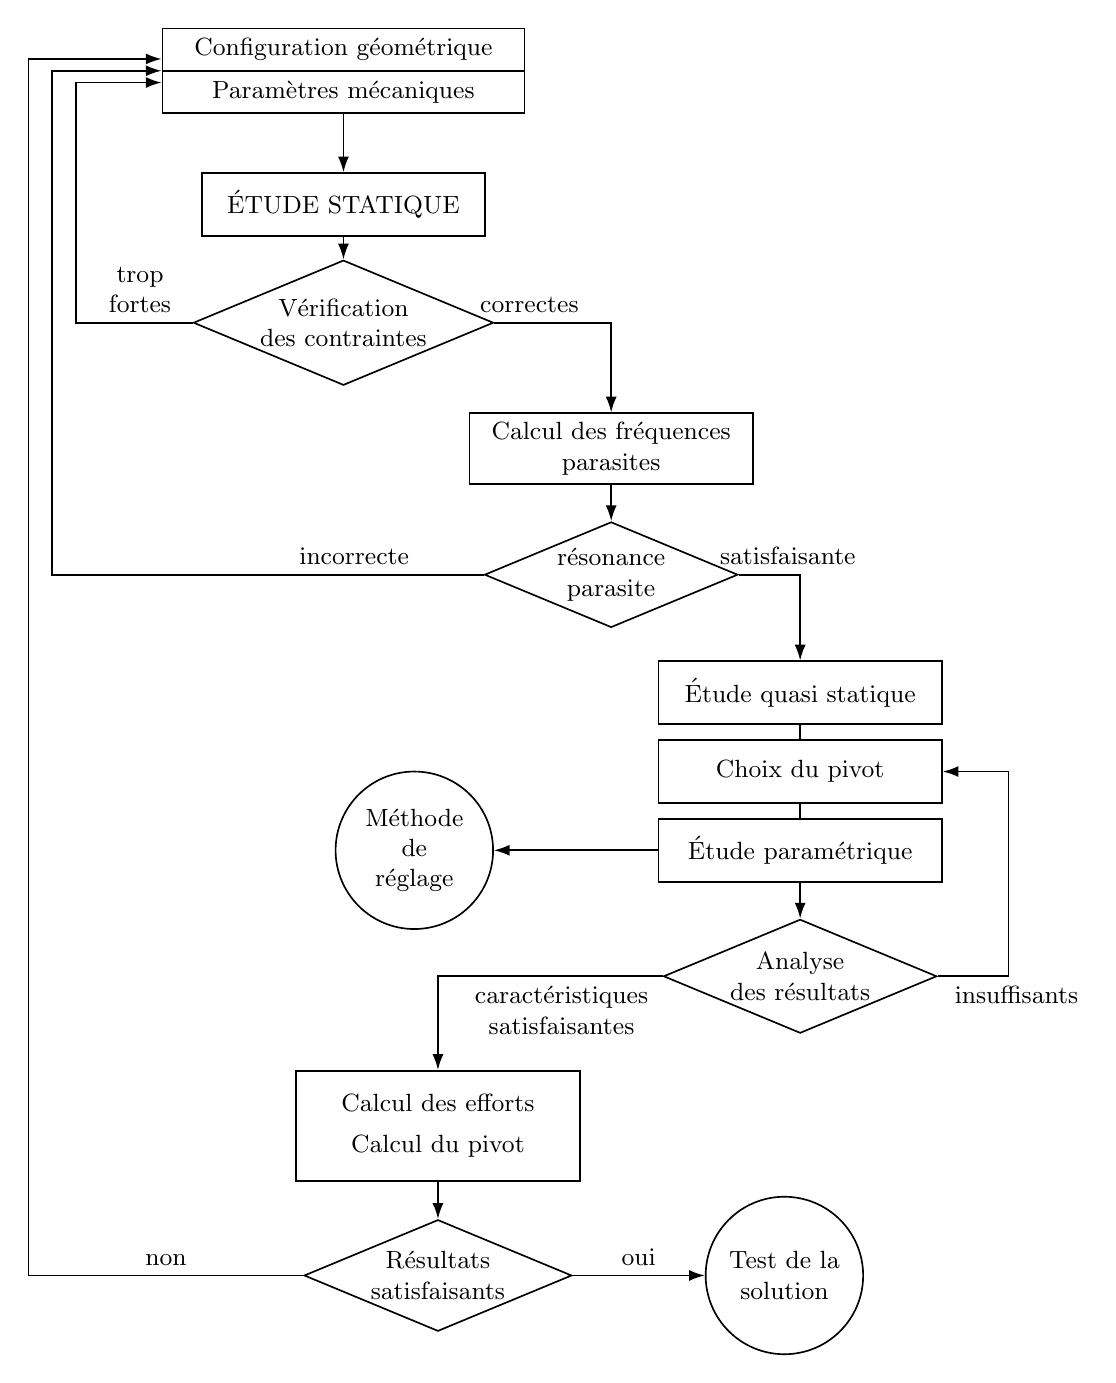
\begin{tikzpicture}[font=\small, node distance=8mm,
    etape/.style={draw, minimum width=3.6cm, minimum height=8mm, align=center, fill=white},
    test/.style={draw, diamond, aspect=2.4, inner sep=1pt, align=center, fill=white},
    rond/.style={draw, circle, minimum size=2cm, align=center}]
  \node[draw, rectangle split, rectangle split parts=2, minimum width=4.6cm, align=center]
    (cfg) at (0,0) {Configuration géométrique \nodepart{two} Paramètres mécaniques};
  \node[etape] (stat) at (0,-1.7) {ÉTUDE STATIQUE};
  \node[test] (verif) at (0,-3.2) {Vérification\\des contraintes};
  \node[etape] (freq) at (3.4,-4.8) {Calcul des fréquences\\parasites};
  \node[test] (reso) at (3.4,-6.4) {résonance\\parasite};
  \node[etape] (quasi) at (5.8,-7.9) {Étude quasi statique};
  \node[etape] (choix) at (5.8,-8.9) {Choix du pivot};
  \node[etape] (param) at (5.8,-9.9) {Étude paramétrique};
  \node[rond] (regl) at (0.9,-9.9) {Méthode\\de\\réglage};
  \node[test] (ana) at (5.8,-11.5) {Analyse\\des résultats};
  \node[etape, minimum height=14mm] (eff) at (1.2,-13.4) {Calcul des efforts\\[4pt]Calcul du pivot};
  \node[test] (res) at (1.2,-15.3) {Résultats\\satisfaisants};
  \node[rond] (essai) at (5.6,-15.3) {Test de la\\solution};
  % flux principal
  \draw[->] (cfg) -- (stat); \draw[->] (stat) -- (verif);
  \draw[->] (verif.east) -- node[above, pos=0.3] {correctes} (verif.east -| freq) -- (freq);
  \draw[->] (freq) -- (reso);
  \draw[->] (reso.east) -- node[above, pos=0.8] {satisfaisante} (reso.east -| quasi) -- (quasi);
  \draw (quasi) -- (choix) (choix) -- (param);
  \draw[->] (param) -- (ana);
  \draw[->] (param.west) -- (regl.east);
  \draw[->] (ana.east) -- node[below right, pos=0.1] {insuffisants} ++(0.9,0) |- (choix.east);
  \draw[->] (ana.west) -- node[below, pos=0.45, align=center] {caractéristiques\\satisfaisantes} (ana.west -| eff) -- (eff);
  \draw[->] (eff) -- (res);
  \draw[->] (res.east) -- node[above] {oui} (essai);
  % retours
  \draw[->] (verif.west) -- node[above, pos=0.45, align=center] {trop\\fortes} (-3.4,-3.2) |- ([yshift=-1.5mm]cfg.west);
  \draw[->] (reso.west) -- node[above, pos=0.3] {incorrecte} (-3.7,-6.4) |- (cfg.west);
  \draw[->] (res.west) -- node[above] {non} (-4.0,-15.3) |- ([yshift=1.5mm]cfg.west);
\end{tikzpicture}
\end{document}
